\documentclass[border=8pt]{standalone}
\usepackage{pgfplots}
\pgfplotsset{compat=1.18}
\begin{document}
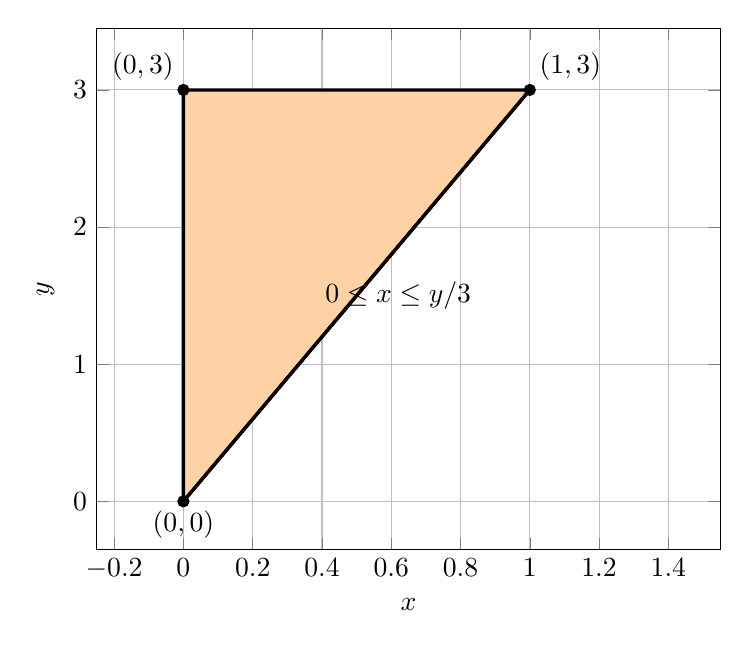
\begin{tikzpicture}
\begin{axis}[
  width=9.5cm, height=8.2cm,
  xlabel=$x$, ylabel=$y$,
  xmin=-0.25, xmax=1.55, ymin=-0.35, ymax=3.45,
  grid=major,
  enlargelimits=false,
]
% filled triangular base region : 0<=x<=y/3, 0<=y<=3
\addplot[fill=orange!35, draw=black, very thick] coordinates {(0,0) (0,3) (1,3)} -- cycle;
% the line y=3x emphasised
\addplot[very thick, domain=0:1, samples=2] {3*x};
\node at (axis cs:0.62,1.5) {$0\leq x\leq y/3$};
\node[anchor=north] at (axis cs:0,0) {$(0,0)$};
\node[anchor=south east] at (axis cs:0,3) {$(0,3)$};
\node[anchor=south west] at (axis cs:1,3) {$(1,3)$};
% mark the corner points
\addplot[only marks, mark=*, black] coordinates {(0,0) (0,3) (1,3)};
\end{axis}
\end{tikzpicture}
\end{document}
